\chapter{绪论}
云计算在赋能海量数据上聚类应用的同时,也带来了数据泄露的风险,引起人们的广泛关注。
如何在提供便捷的云计算服务的同时,保护用户的数据安全成为了当今学术研究的热门问题,极具现实意义。
本章首先介绍云环境下的聚类应用的相关背景,然后阐述设计隐私保护聚类方案的重要意义,最后总结文章主要工作内容及创新点,并给出了论文整体组织结构。

\section{研究背景与意义}
% 直接一把子照搬开题报告!
随着现代社会数字化的不断演进,数据使用量呈指数级增加,个人和小型组织越来越难以在内部计算机服务器上维护所有重要信息、运行大型程序和系统。为解决这些问题,云计算应运而生。自云计算在2006年被提出后,它就被认为是能够推动下一代互联网革命的技术,并迅速成为了研究领域的热门探索方向\cite{sadiku2014cloud}。
云计算既可以指在网络上提供的应用服务,也可以指数据中心中提供这些服务的硬件和系统软件,它能够将互联网中众多计算资源进行管理和调度,根据用户的计算需求提供服务,它的运行原理和基于Web的电子邮件客户端类似,允许用户访问系统的所有功能和文件,但是无需将系统的大部分内容保存在自己的计算机上。
此外,云计算在各个领域都有广泛且深刻的应用(如图\ref{img_cloud}),例如在智能教育领域,为学生提供在线课程和为老师提供授课工具;在智慧医疗领域,为医生和患者提供远程诊疗、电子病例和医疗数据分析等功能;在商业领域,为企业组织提供电子商务、市场分析以及资源规划等功能。

\begin{figure}[htbp]
	\centering
	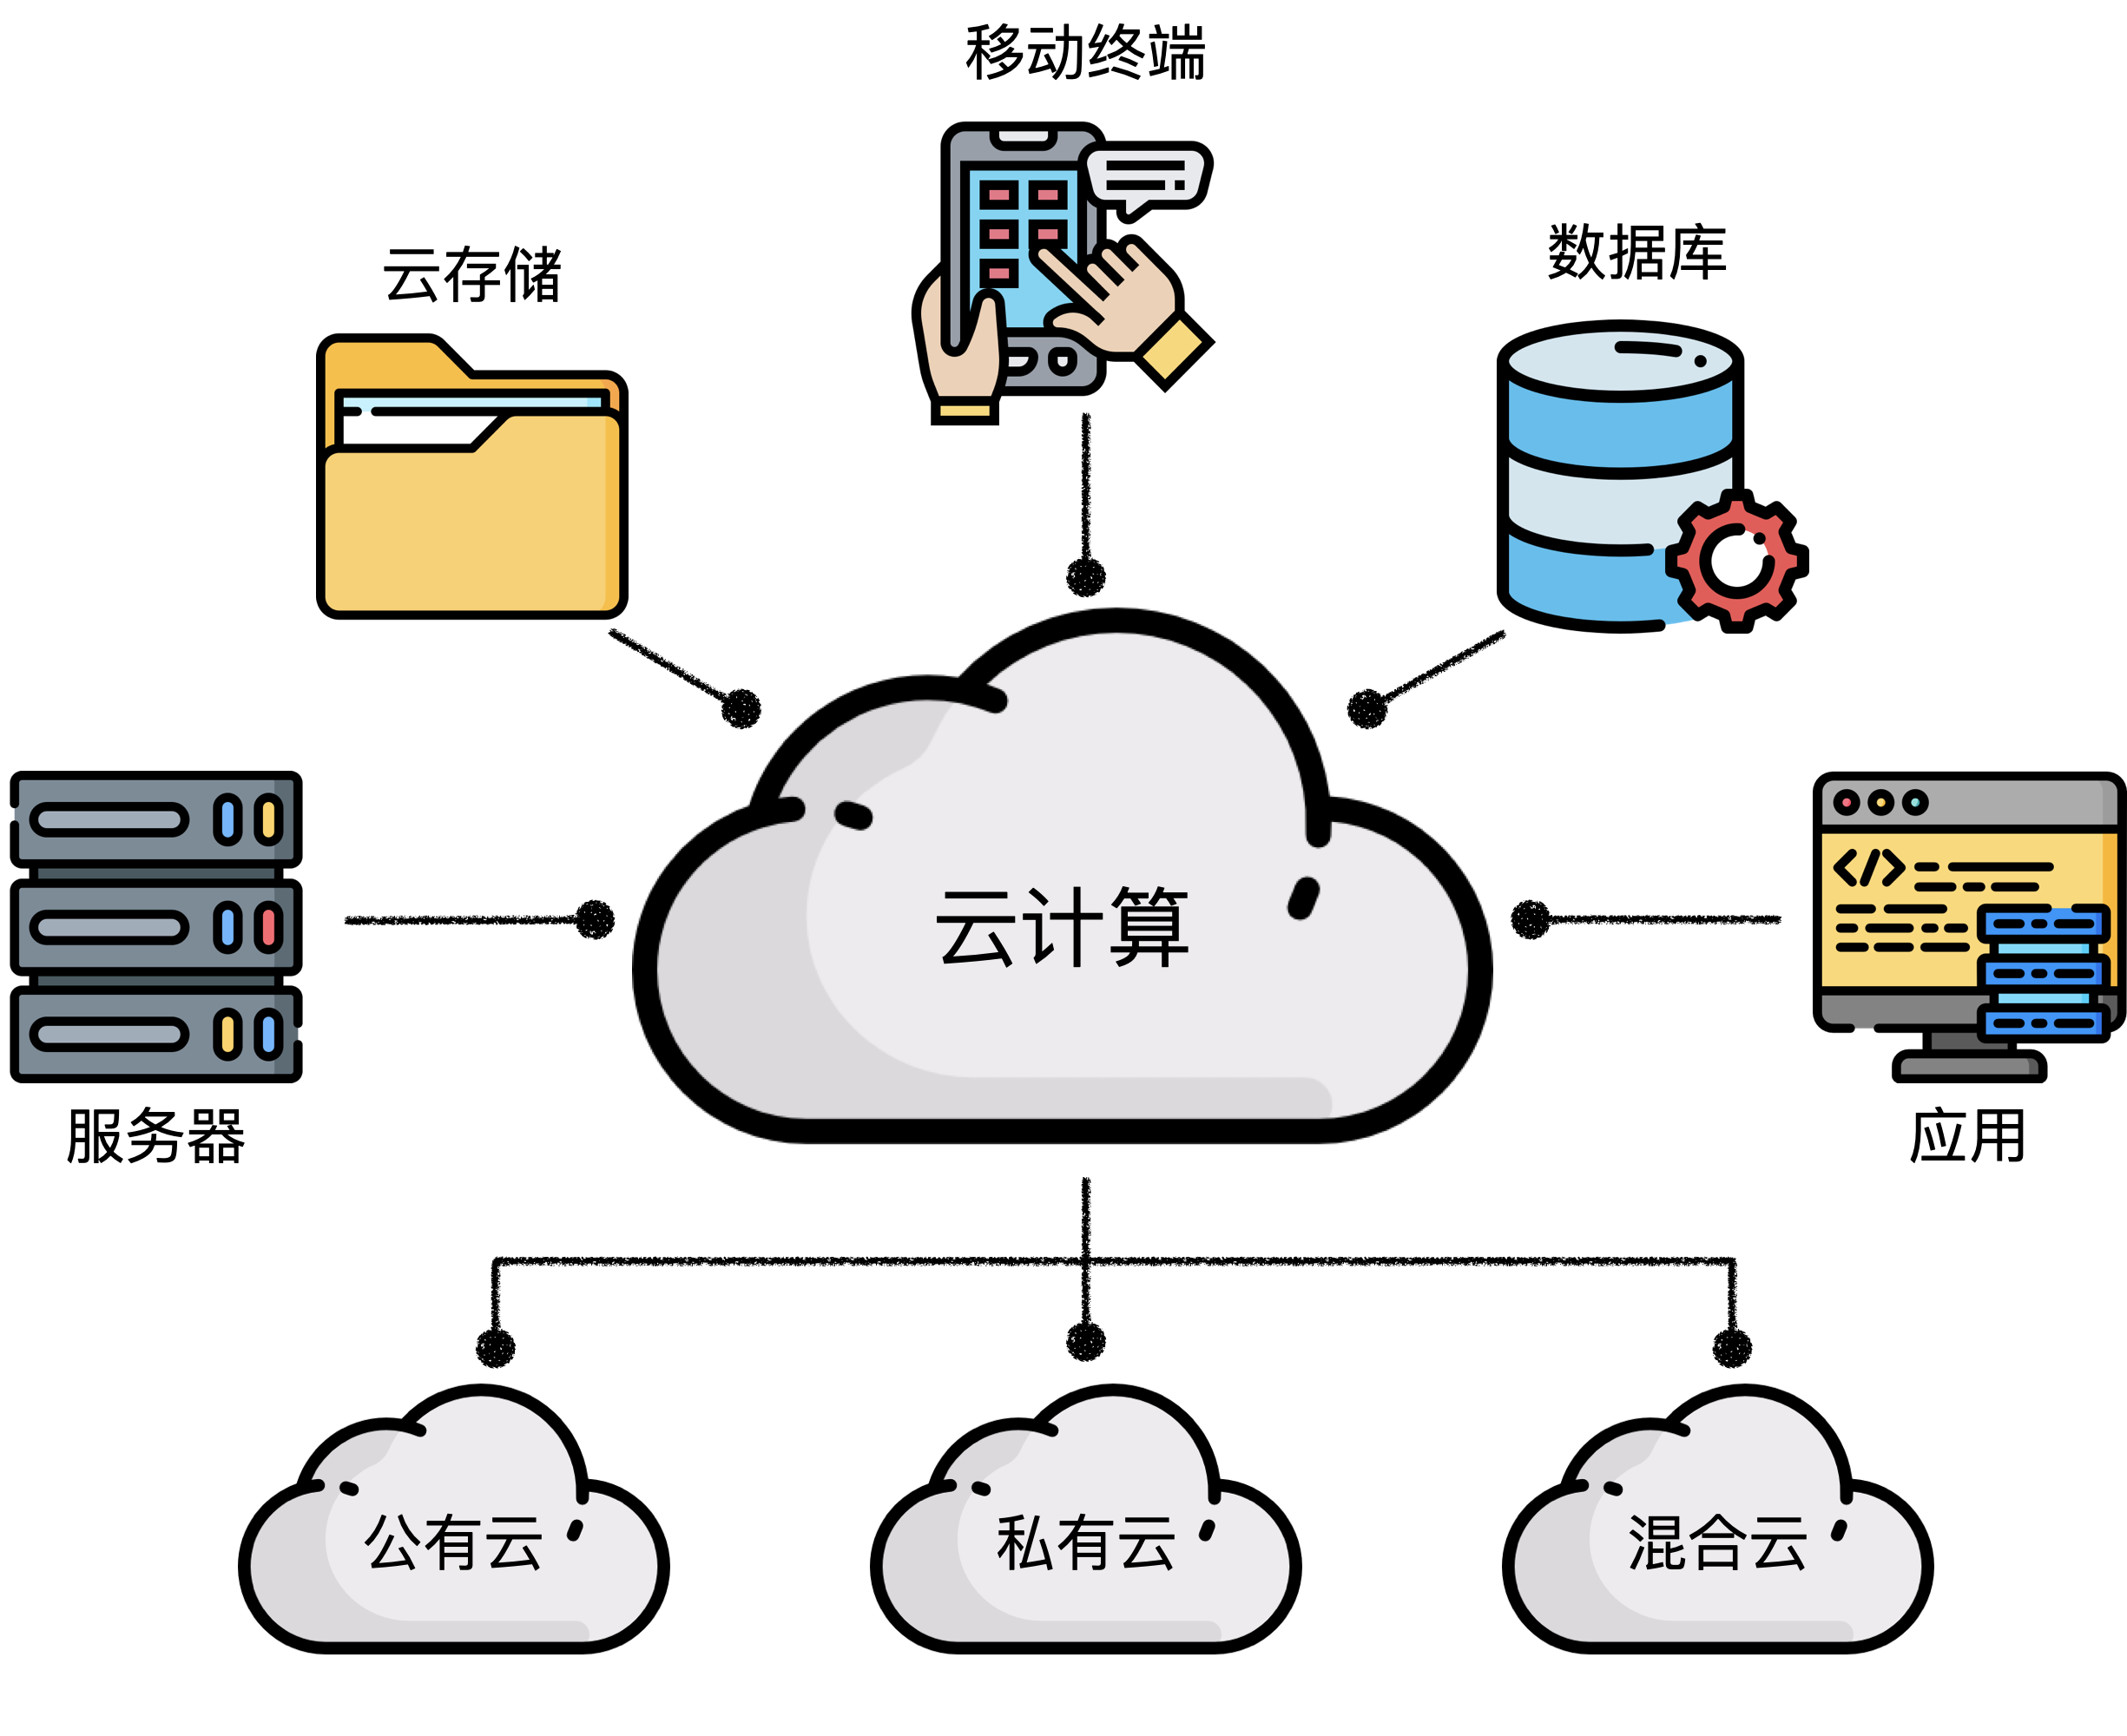
\includegraphics[width=0.55\linewidth]{img/cloudarchi.png}
	\caption{云计算架构}
	\label{img_cloud}
\end{figure}

云计算具有经济实惠、按需服务、方便、通用、多租户、灵活以及稳定等特点,它主要提供了三种服务交付模式,如图\ref{img_saas}所示,分别是基础设施即服务(IaaS)、平台即服务(PaaS)以及软件即服务(SaaS)。
IaaS将计算机硬件(例如网络存储、虚拟机、数据中心、处理器和内存)视为一种服务,无需大量资金和时间即可提供可扩展基础架构。同时,IaaS还可以用于构建防火墙,虚拟机监控和其他安全领域\cite{manvi2014resource}。
%IaaS的优势在于能够节省用户购买和维护物理设备的成本和时间,提高资源利用率和可扩展性,实现灵活的部署和迁移。常见的应用场景有网站托管、系统容灾、大数据分析以及测试开发环境等等。
PaaS以开发工具、框架、架构、程序和集成开发环境的形式提供服务。它的优势在于用户可以在云端获取各种开发工具、中间件以及数据库等资源,用户无需自己购买相关软硬件,关注开发的逻辑和功能即可。
%Paas的架构通常采用容器化技术,即将应用程序打包成可移植的容器,通过互联网提供给用户。但在快速发展的同时,PaaS还面临着诸多挑战,例如生命周期开发和底层基础设施安全等问题\cite{rani2014comparative}。
SaaS是远程计算服务的集合,它使得第三方供应商能够远程部署应用程序。云计算客户可以在云基础设施上通过网络获取云服务提供商的应用程序\cite{antonopoulos2010cloud}。
%SaaS的典型应用场景有办公软件、电子邮件以及企业资源规划等。其架构通常采用多租户技术,将同一套应用程序提供给多个用户使用,每个用户只能看到自己的数据和配置,提高了资源利用率和扩展性,降低了运营成本。

\begin{figure}[htbp]
	\centering
	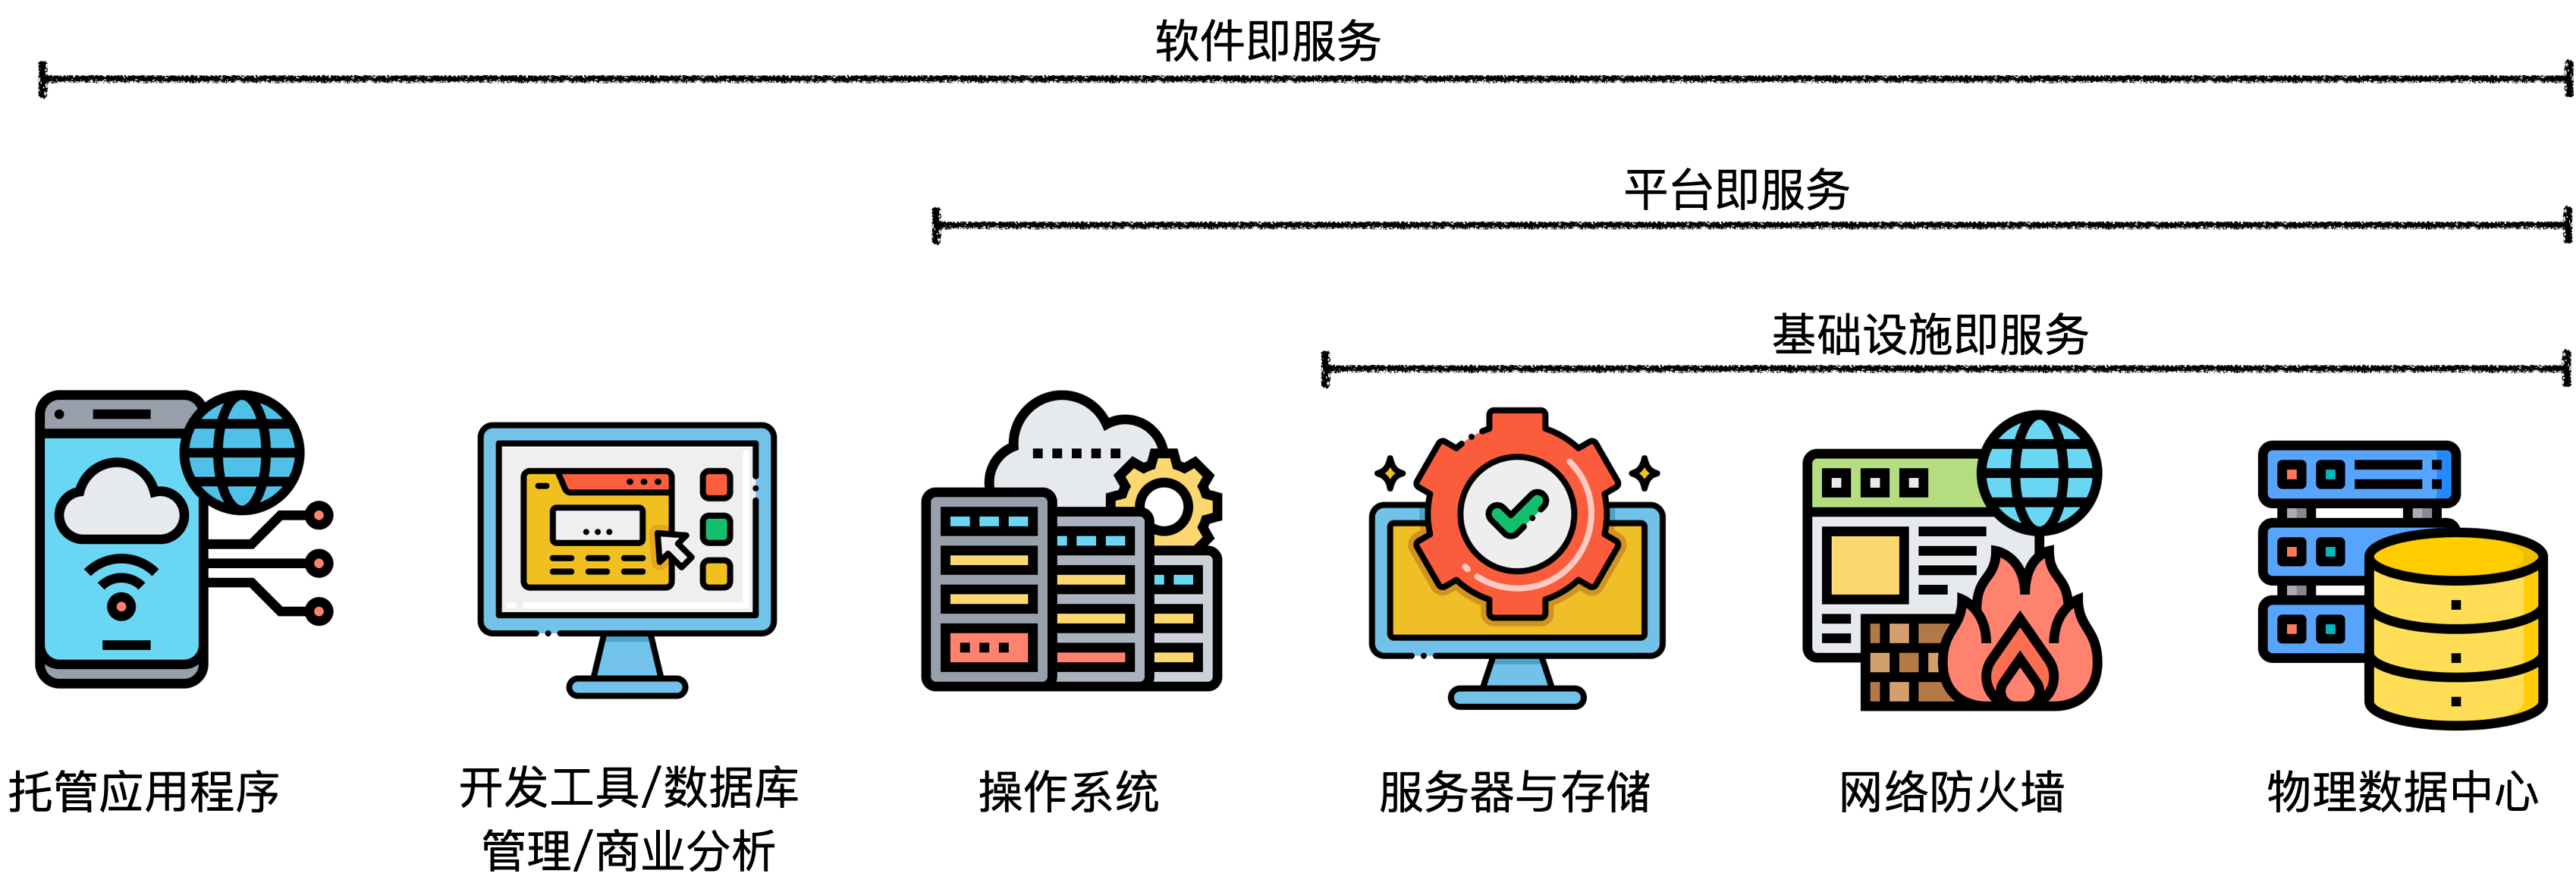
\includegraphics[width=1.0\linewidth]{img/cloudservice.png}
	\caption{云计算服务交互模式}
	\label{img_saas}
\end{figure}

近年来,云计算场景下出现了一种新的服务类型,机器学习即服务(Machine Learning as a Service,MLaaS)\cite{ribeiro2015mlaas}。随着研究的发展和设备的进步,机器学习从学术研究落地到生活的方方面面,但是大多数机器学习任务对于设备的性能要求较高,需要存储海量的数据才能取得较好的结果。大型公司有能力承担设备费用,利用机器学习的便利开展各种各样的研究与服务,但是资源有限的小公司和个人的需求常常难以被满足。

MLaaS基本上是一组基于云的工具的总称,这些工具以一种全新的方式支持科学家和数据工作者的日常工作,它们支持协作、版本控制、并行化和其他比较复杂的任务。
此外,较大的云服务供应商提供简单明了的方法来将他们的MLaaS服务与其他工具集成,方便用户进行自动化部署以及执行机器学习任务。
MLaaS包含很多种类,例如自然语言处理、图像和视频分析、计算机视觉、语音识别以及数据挖掘等等。
随着机器学习技术的发展和进步,提供MLaaS的公司数量也在增加,主流的公司包括微软的Azure和谷歌的Google Cloud ML等等。在MLaaS中,海量的数据需要被上传到云计算中心,这一过程也被称之为外包计算。
由于用户在数据上传后失去了对数据的完全控制,因此会更加关心数据隐私问题。云计算服务模型的复杂性、实时性、数据的多元异构以及终端资源有限等特点使得传统的数据隐私保护方法无法直接用来保护云计算中的大量数据\cite{hunt2018chiron}。

在2018年,脸书被爆出隐私泄露丑闻,近5000万选民的个人资料被泄露,据称被某政治咨询公司所使用。这一丑闻的发展不仅使得该公司的市值减少数十亿美元,同时还引发了公众的强烈不满和质疑,由此可见保护数据的隐私安全无论是对公司还是对用户都有深远意义。
将一些敏感的数据进行外包以获取机器学习的结果可能会引发隐私泄漏问题,特别是在金融以及医疗领域。以医疗影像识别为例,在对数据不进行任何处理的前提下交付给云服务器进行训练,会直接造成用户私密医疗数据的泄漏,引发公众恐慌。即便是对用户的数据进行了简单的脱敏,模型训练的中间结果也可能会被恶意利用以获取信息。以K-means聚类为例,虽然原始数据经过加密,但是中间结果,例如聚类簇的大小,能够直接揭露具有某种特征的群体有多少人以及数据的分布特点,有研究表明可以通过一些手段从中间结果恢复原始数据\cite{liu2021when}。因此,如何进行安全的外包计算,在维护用户数据安全的同时,正确的获取外包机器学习任务的结果成为一个研究热点。

聚类(Clustering)是一种非常流行的无监督机器学习技术,它能够将相似的输入元素划分到同一个簇(Cluster)中。
聚类的应用场景非常广泛,从业务分析到医疗保健等诸多领域。在这些应用场景中,敏感信息在被正确聚类的同时,也不应该被泄漏。此外,现在经常需要将不同来源的数据组合起来进行训练以提升聚类结果的质量,庞大的数据量对资源有限的用户带来巨大的压力,因此,通常需要将复杂的计算外包给强大的云服务器进行处理,这就要求设计有效的外包隐私保护聚类方案\cite{ahmed2020k}。
目前,为了保护聚类过程中输入的敏感数据的安全性,已经有了诸多研究成果,涵盖各个方面。在设计隐私保护聚类协议时,通常基于两个不同的场景,即多方计算(图\ref{scen2})与外包计算(图\ref{scen1})。
\begin{figure}[htbp] %[htbp]
	\begin{minipage}[t]{0.45\linewidth}
		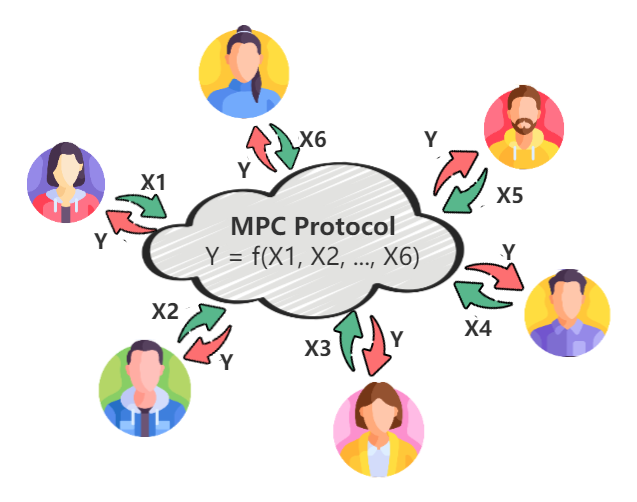
\includegraphics[width=\linewidth]{img/mpc.png}
		\caption{多方计算}
		\label{scen2}
	\end{minipage}
	\hfill
	\begin{minipage}[t]{0.45\linewidth}
	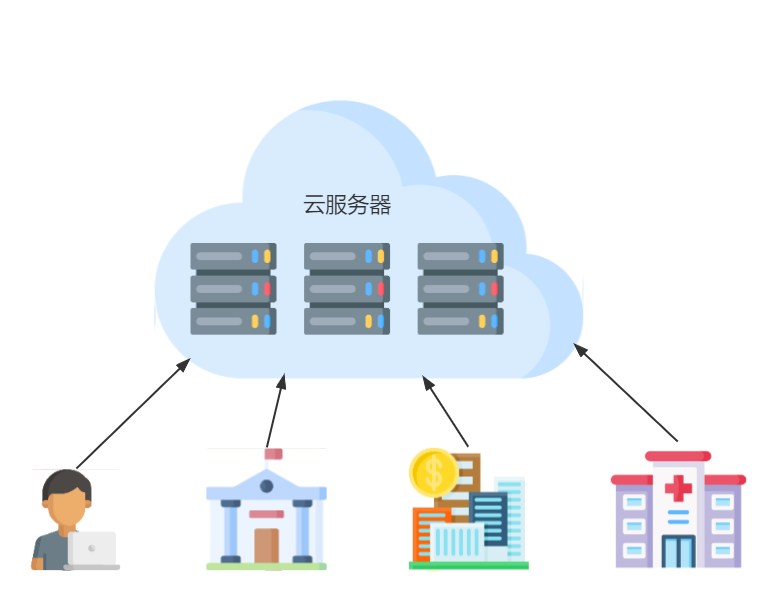
\includegraphics[width=\linewidth]{img/outsource.png}
	\caption{外包计算}
	\label{scen1}
	\end{minipage}
\end{figure}

在多方计算的场景下\cite{cramer2015secure},两个及两个以上的数据所有者共同执行安全计算协议,除了输出之外的任何内容都不会泄漏给彼此,比较常见的是两方计算。同时,一些研究也会在模型设计中引入半诚实参与方(通常是服务器)来辅助计算。
相对应的,另一种场景则是外包计算\cite{li2018privacy},一个或多个数据所有者将计算(或存储)外包给其他参与方,并假设这些参与方可以为数据所有者进行聚类而无需知道关于输入数据的任何信息。由于外包计算旨在使用外部资源,数据所有者通常不应该参与协议的执行,并处于离线状态,但是这一要求通常难以完全实现。
值得一提的是,一些多方计算协议也可以用于外包计算场景,只需要数据所有者在多个不共谋的参与方之间秘密共享自己的数据,然后多个不共谋的参与方在秘密共享数据上执行安全协议实现聚类。但是,多方计算协议是否支持外包计算很大程度上取决于中间协议的设计,如果数据持有者需要在聚类过程中进行大量的明文计算或者在中间对数据进行解密,那就很难将协议转换到外包计算的场景中。

外包计算和多方计算各有其优势和缺点,对于资源有限的用户来说,外包计算更加具有实际意义和价值,能够有效的减轻用户的资源负担。基于外包计算的安全计算方法已有诸多研究,但是完全安全的隐私保护外包聚类方案通常效率较低,即便是在性能较好的服务器上也需要花费难以接受的时间才能获得最终结果,效率较高的方案通常会牺牲一定的安全性,例如泄漏簇大小、簇中心这样的中间计算结果,带来一些隐私安全问题。因此如何设计出安全又高效的外包隐私保护聚类方案值得深入研究和探索。

综上所述,本文以云计算下的隐私保护外包聚类为主要应用场景,深入分析其面临的基本问题和技术难点,以设计兼具效率与安全的方案为主要目的,针对典型的聚类算法(K-means和DBSCAN)展开研究,提出了完善的隐私保护方案,并通过理论分析和真实数据集测试,验证所述方案的安全性、高效性和正确性。通过本文的研究,期望能够为资源有限的用户提供一种可行的隐私保护外包聚类方法,为云服务提供商与独立用户提供合作的桥梁,使得用户能够专注于数据的挖掘分析,云服务提供商进一步提高资源利用率,各司其职,物尽其用,让更多人无需顾虑数据安全更加放心的享受科技进步带来的生活水平提升。

\section{云环境下聚类中隐私保护问题概述}
%本节首先介绍聚类的概念和云环境下聚类的典型应用场景,然后讨论云环境下聚类都存在哪些具体的数据安全与隐私问题,最后讨论针对上述问题目前已有的解决方案和技术手段。
本节首先给出云环境下聚类研究综述,分别详细介绍了云计算、聚类算法以及云环境中聚类算法的应用,然后介绍云环境下聚类应用中存在的数据安全问题。基于上述内容,总结归纳了隐私保护聚类研究中常用的技术手段,并探讨了隐私保护聚类方案的设计目标。
\subsection{云环境下聚类相关研究概述}
%本小节首先介绍云计算的基本概念和常见应用场景,然后对机器学习中的聚类技术展开介绍,最后介绍云环境下的聚类方案基本应用。
\subsubsection{云计算概述}
云计算是指一种基于互联网的按需提供计算机系统资源,特别是数据存储(云存储)和计算能力,并且无需用户自行采购、配置或管理资源的计算模式,其允许用户通过互联网使用分布在世界各地的服务器上的资源\cite{montazerolghaem2020green}。云计算的部署模型通常可以分为三种,分别是公有云、私有云和混合云。公有云由第三方云服务提供商运营,使用户可以按照特定要求和业务目标安排资源部署。私有云由单个组织构建管理,以非公开的方式托管在本地,具有更强的数据控制、安全和管理功能。混合云是上述二者的结合体,使得用户既能利用公有云服务,同时保持私有云架构中常见的安全和合规功能。

云计算具有灵活性、成本低、高可靠、以及可共享等优点,带给用户巨大的便利,资源有限的用户无需关心如何部署、管理和维护IT基础设施,只需要付费即可获取想要的资源和服务。这项技术解放了用户的双手,使他们能够专注于本领域的研究与工作,提升效率。

\subsubsection{聚类算法概述}
聚类是一种无监督机器学习算法,它能够将一组数据划分到不同的集合中,即簇。簇内部数据相似度较高,簇与簇之间数据相似度相对较低。聚类在实际的应用中非常广泛,常见于数据挖掘分析、生物信息处理、文本挖掘提取以及图像处理等领域。通过聚类能够找到不同数据集合特有的模式与结构,挖掘隐藏在背后的信息,从而进行分析和进一步处理。

常见的聚类算法包括:
\begin{compactitem}
	\item
	\textbf{基于划分的聚类方法:}也叫基于分区的聚类或基于距离的聚类,核心思想为假定数据集有$ n $个样本,在满足样本间距离的前提条件下,最少将其划分为$ k $个簇。簇内数据尽可能相似,不同簇的数据尽可能不相似。常见的基于划分的聚类方法包括K-means算法和K-medoids算法。
	\item
	\textbf{基于层次的聚类方法:}将数据对象划分为层次结构可以帮助我们更好地理解聚类结果,同时也方便选择合适的聚类数量。在聚类过程中,可以采取自顶向下或者自底向上的顺序进行操作。自顶向下也称为分裂,将所有样本当作一个簇,找到最远的两个簇进行分割,直到满足预期条件;自底向上则是将每个点都看成一个独立的簇,找到距离最近的两个簇进行合并,重复迭代直到满足预期。常见的层次聚类算法包括AGNES(聚合层次法)、DIANA(分裂层次法)等,它们在具体实现上各有特点,可以根据具体需求选择合适的算法。%	将数据对象划分为层次结构,可以采取自顶向下或者自底向上的顺序进行操作。自顶向下也称为分裂,将所有样本当作一个簇,找到最远的两个簇进行分割,直到满足预期条件。自底向上则是将每个点都看成一个独立的簇,找到距离最近的两个簇进行合并,迭代重复直到满足预期。常见的聚类算法包括AGNES、DIANA等。
	\item
	\textbf{基于密度的聚类方法:}根据样本的密度分布进行聚类,通过样本密度反映数据之间的可连接性,并通过可连接性不断扩展从而产生最终的聚类结果。算法认为密度较高的区域中数据对象属于同一个簇,密度低(包含较少或不包含数据)的区域则形成了簇的边界。该方法能够发现任意形状和大小的簇,对噪声不敏感。常见的算法有DBSCAN、OPTICS等。
	\item
	\textbf{基于网格(Grid)的聚类方法:}将数据空间划分为若干网格单元,并将数据对象映射到网格中,计算每个单元的密度,通过预设阈值来判断网格是否为高密度单元,邻近的稠密单元进行合并构成了簇。该方法可以大大减小聚类计算复杂度,但是对网格的划分方式要求较高。典型的算法包括STING、CLIQUE等。
	\item
	\textbf{基于模型的聚类方法:}该方法的核心思想为假设每个簇都符合某种概率模型,例如正态分布,然后借助最大似然估计法或者贝叶斯推断来估计模型参数并划分数据到所属簇中。该方法能够得到明确的聚类结果,但是对模型和参数的选择要求较高。常见的算法有EM、GMM等。
	%	\item \textbf{K-means:}是一种最为常见的聚类算法,基于欧式距离衡量相似度,不断迭代直到算法收敛获取划分结果。首先,随机选择$ k $个簇中心,然后遍历集合中所有数据,求解到$ k $个簇中心的距离,并据此划分到最近的簇中。最后根据划分结果,更新簇中心为簇内数据的平均值,重复上述过程直到满足判定收敛的条件。
	%	\item \textbf{层次聚类:}是通过对数据集在不同的层次进行划分,按照自顶向下或者自底向上的步骤,逐步形成树形结构的聚类算法。自底向上的方式将每一个原始数据看成一个单一的聚类,然后不断合并从而成为大的聚类。而自顶向下的方式则是将所有数据看作一个大的聚类,通过不断分割直到每一个单一数据被划分。
	%	\item \textbf{DBSCAN:}是一种典型的基于密度的聚类算法,它将簇定义为密度相连的数据点的最大集合,将满足要求的高密度区域划分为簇,能够发现任意形状的聚类,并识别噪声点,并对异常点不敏感。
\end{compactitem}

综上所述,聚类算法的划分一般可以基于划分、密度、网格和模型等方式。不同的具体聚类算法各有优缺点和适用场景。下面在表格\ref{s1_table_clustering}中,给出几个常见的聚类算法,以及它们在应用数据的规模、对噪声的抗干扰能力、适合的数据形状和算法效率方面的特点。
\begin{table}[htbp]
	\centering
	\renewcommand{\arraystretch}{1.3}
	\caption{常见聚类算法比较}
	\label{s1_table_clustering}
	\scalebox{1.0}{
		\begin{tabular}{c|c|c|c|c}% 通过添加 | 来表示是否需要绘制竖线c|
			\hline  % 在表格最上方绘制横线
			算法类型 & 可用于大规模 & 对噪声抗干扰性 & 适合形状 & 算法效率 \\%&SKD
			\hline % 在表格最下方绘制横线
			K-means  & 是           & 较差           & 球形     & 很高     \\
			\hline
			DBSCAN   & 是           & 较好           & 任意形状 & 一般     \\
			\hline
			BIRCH    & 否           & 较差           & 球形     & 很高     \\
			\hline
			CURE     & 是           & 很好           & 任意形状 & 较高     \\
			\hline
		\end{tabular}
	}
\end{table}

本文主要基于K-means和DBSCAN聚类算法展开隐私保护方案相关研究。二者在对噪声的抗干扰性、适合的数据集形状以及算法效率方面存在一些区别。图\ref{clu_difference}中可以看到K-means和DBSCAN在不同数据集上聚类结果的区别。
五个测试数据集中包含了多种不同形状的簇,可以看到K-means算法仅在第四列数据集上划分效果较好,该数据集包含的簇形状均为凸型,而DBSCAN则在所有测试数据集上划分效果更好,能够发现任意类型的簇,并检测出异常值。


\begin{figure}[htbp]
	\centering
	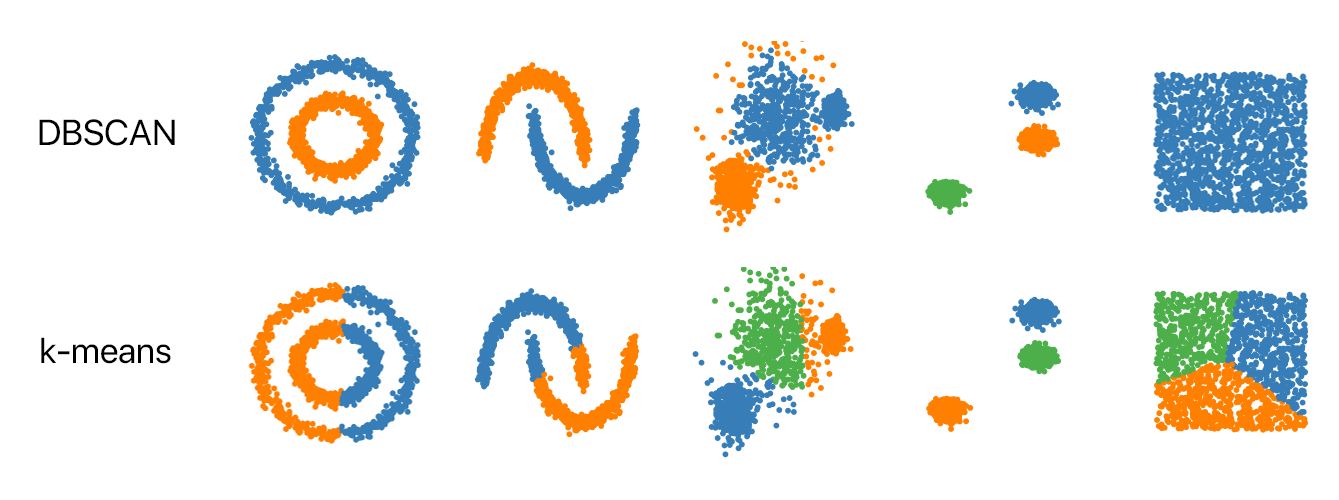
\includegraphics[width=\linewidth]{img/difference.png}
	\caption{DBSCAN与K-means聚类结果对比}
	\label{clu_difference}
\end{figure}

\subsubsection{云环境下的聚类应用}
\label{juleiyanjiu}
云环境下聚类算法的实施通常依赖于外包计算这一计算模式,即将计算任务和数据交给云服务提供商进行处理。外包计算的流程主要包括数据准备、任务分配、计算处理以及结果返回。它具有节省用户的计算资源、提升计算效率以及降低成本等优点。从用户角度来看,外包聚类计算的应用主要可以细分为两种,分别是单用户上传数据聚类和多用户分别上传数据进行联合聚类。

单用户外包聚类,例如高校的学生老师或是小型的研究开发团队,通常希望能够对指定的数据集进行聚类,获取结果用于后续挖掘分析。这些用户拥有的计算和通信资源通常有限,难以在本地机器上对大型数据集进行处理,因此会选择将数据上传至云平台后,以外包计算这一形式获取结果。

多用户协同外包聚类,例如银行或医院等机构,因自身业务的开展,会产生极具研究价值的数据,深入挖掘分析这些数据,可以为医疗影像研究和用户信用评估等方面的研究提供指导。然而,独立机构产生的数据量有限,海量数据上的聚类通常效果更好,聚类结果价值更高。
但是上述机构对数据安全的要求较高,通常期望能够在不泄露自身数据的前提下,获取协同聚类的结果。
因此这些机构倾向于将数据加密后上传到云平台上进行聚类。以医院为例,医疗影像常用于各种疾病的辅助诊疗,联合多个医疗机构在大量数据上进行挖掘分析能够提取出各种特征用于研究,造福人类。

综上所述,外包计算中聚类的数据来源有所区别,但算法收敛后聚类结果以相同的方式通过互联网传递回用户手中以进行后续的研究分析。值得一提的是,不同聚类场景带来的差异对隐私保护方案的设计也会产生一定的影响。多用户协同的场景无法联合所有明文数据进行处理,单用户上传数据的场景则可以对原始数据做出多种处理获取信息辅助外包计算。
% 感觉好像并不是很必要
%两种情况,资源受限的独立用户需要外包训练,不同组织机构需要上传数据联合聚类
%聚类的实施通常需要云计算平台提供帮助与支持,尤其是在需要处理大型数据集时。本文主要考虑以下两种云环境下的聚类应用。
%
%一方面,独立用户,例如高校的学生老师或是小型的研究开发团队,他们通常希望能够对指定的数据集进行聚类,获取结果用于后续挖掘分析。这些用户通常计算资源受限,难以在本地机器上对大型数据集进行处理,因此会选择将数据上传至云平台后,以外包计算这一形式获取结果。
%
%另一方面,一些组织机构,例如银行或医院,因自身业务的开展,会产生极具研究价值的数据,深入挖掘分析这些数据,可以为医疗影像研究和用户信用评估等方面的研究提供指导。然而,独立机构产生的数据量有限,海量数据上的聚类通常效果更好。因此这些机构倾向于联合其他机构,将数据上传到云平台上共同聚类。以医院为例,医疗影像常用于各种疾病的辅助诊疗,通过对这些数据进行挖掘分析能够提取出各种特征用于研究,造福人类。
%
%综上,云环境下的聚类场景通常可以划分为两类:一种是资源受限的独立用户上传自身数据或指定开源数据集,进行聚类获取结果;另一种则是,多个用户(组织机构之间联合)上传数据到云平台联合进行聚类,获取结果以进行后续挖掘分析。
\subsection{云环境下聚类中的隐私问题}
本小节主要就云环境下外包聚类计算中存在的隐私问题展开讨论,并总结了几种现有的典型隐私保护技术。如前所述,在外包计算中,用户需要将数据全部上传至云平台,云服务器利用这些数据进行聚类训练,并回传结果。

若外包计算模式下,云平台接收的数据并非全部源自网络公开数据集,而是有可能来自独立用户或者组织机构上传的数据。在这种情况下,数据本身通常具有较高的隐私保护要求。
例如,医疗机构希望借助云计算强大的计算能力和海量的存储空间来对其医疗影像信息展开挖掘分析,从而在诊疗中辅助医生进行判断和诊断,其外包的数据通常包含患者的敏感信息,例如年龄、性别、籍贯、医疗影像以及相关医学检查结果。
智能穿戴设备需要获取用户的各种私密数据,如心率、步数、运动状态以及睡眠状态等内容进行分析然后将结果反馈给用户。
一旦发生数据泄露,会造成巨大损失。
此外,即便是对原始数据进行了加密操作,云平台在这些密文数据上进行聚类获取结果的同时,还会获取若干中间计算结果,这些数据的安全性也要纳入考虑。因此,对于云环境下隐私保护方案中数据安全问题的研究,需要考虑原始数据、中间结果以及划分结果等多个方面。

\subsection{隐私保护聚类技术手段}
云环境下隐私保护聚类方案的一大难点在于,如何在保证原始数据以及中间结果隐私性的前提下,完成安全高效的聚类运算。当下,聚类研究中常见的隐私保护技术手段大体上可以分为数据扰动、差分隐私、同态加密以及安全多方计算。本节将分别介绍上述几种技术的基本原理以及各自的优缺点。

\subsubsection{数据扰动}
数据扰动(Data Perturbation)是一种隐私保护方法,允许在不泄漏原始数据信息的情况下,对数据进行一定的扰动,从而达到保护隐私的目的。数据扰动方式主要可以分为两种类型:

\begin{compactitem}
	\item \textbf{概率分布方式:}是数据扰动技术中一种重要手段,通过调整数据的概率分布来保护敏感信息。通常从相同的分布样本中或者从分布本身中获取数据进行替换。常见的实现方式有拉普拉斯机制、高斯机制以及指数机制。但是若数据分布比较复杂,则难以用简单的概率分布来进行扰动。同时噪声的大小和分布需要根据具体的应用场景和应用特征来进行选择。
	\item \textbf{数值失真方式:}借助加法、乘法或其他随机过程扰乱数据。其中,添加加性随机噪声,使得攻击者无法获取单个数据的原始信息,但是由于没有影响数据的分布特征,因此仍能够通过分析挖掘出数据相关有效信息。乘性扰动则是指利用数据投影等方法,将原始数据映射到低维空间,例如可以使用随机映射技术将数据映射到一个随机选择的子空间中。
\end{compactitem}

综上所述,数据扰动技术实施较简单,引入开销较小,适用场景广泛,但是存在着安全性较低、影响数据质量等问题。具体使用中需要权衡数据隐私性和数据准确性进行取舍。

\subsubsection{差分隐私}
Dwork等人\cite{dwork2006differential}在2006年提出一种全新的隐私定义,即差分隐私。它能够确保在数据集合中添加或者删除某项内容,不会显著影响任何相关数据分析的结果\cite{dwork2008differential},将隐私泄露风险控制在可接受范围内,恶意攻击者无法通过观察运算结果来获取精确的单个数据信息。目前已有较多关于差分隐私的研究和应用,实际场景中通常采取本地化差分隐私技术保护隐私安全,苹果的iOS系统\cite{team2017learning}、谷歌的Chrome浏览器\cite{erlingsson2014rappor}以及微软的Windows系统\cite{ding2017collecting}均已应用这项技术。
差分隐私的具体定义\cite{dwork2011firm}如下:

\begin{definition}
	设有随机算法$ \varGamma $,$ \varGamma $所有可能输出构成的集合为$ O_{\varGamma} $。对于任意两个邻近数据集$ D $和$ D' $以及$ O_{\varGamma} $的任何子集合$ S_{\varGamma} $,若算法$ \varGamma $满足
	\begin{equation}
		\operatorname{Pr}\left[M(D) \in S_M\right] \leq \exp (\varepsilon) \times \operatorname{Pr}\left[M\left(D^{\prime}\right) \in S_M\right]
	\end{equation}
	则称算法$ \varGamma $ 能够提供$ \epsilon$-差分隐私保护。
\end{definition}

其中参数$ \epsilon $称为隐私保护预算,它用来控制算法$ \varGamma $在两个相邻数据集上取得相同输出的概率比值,反映了$ \varGamma $提供的隐私保护水平,当$ \epsilon $越小时,隐私保护的力度越大,需要的噪声越多,$ \epsilon $等于0时,隐私保护水平最高。

通过在原始数据上添加噪声,既保护了隐私又保留了原始数据的统计特征。以数据库查询为例,利用差分隐私技术对数据库进行处理,能够实现数据库中具体某个记录发生变化但不影响数据发布的结果,同时攻击者无法通过观察数据库发布的结果来推测用户的某条记录是否在数据库中,进而实现隐私保护。

使用差分隐私技术能够有效避免数据泄露,保护用户的隐私,通过控制添加噪声的多少,可以在数据的隐私保护与查询结果的准确性之间取得一定的平衡。此外,差分隐私对于数据的保护能力不受具体数据特征的影响,能够用于各种类型的数据和场景。然而差分隐私技术存在一定的局限性,在处理较小数据集时,添加噪声的影响变大,可能会导致数据质量下降,进而影响数据挖掘分析的结果。引入差分隐私,会带来额外的计算和时间成本,降低系统的效率。

综上,差分隐私技术既有隐私保护能力,又有其受限制的地方。在使用这项技术的过程中,需要进行隐私与数据质量之间的平衡,避免数据失真或丢失给研究与应用带来不必要的干扰,同时又要根据数据集的特点和具体的隐私保护要求来设计符合要求的差分隐私保护方案。

\subsubsection{同态加密}
同态加密(Homomorphic Encryption)是一种特殊的加密方式,和经典加密方式不同的是,同态加密允许直接在加密数据上进行计算,而不需要访问密钥。计算的结果仍然处于加密状态,并且可以通过密钥解密,还原计算后的明文结果。其具体定义如下:
\begin{definition}
	若一个加密方案支持如下公式,则称为操作$ \star $上的同态
	\begin{equation}
		D(E\left(m_1\right) \star E\left(m_2\right))=D(E\left(m_1 \star m_2\right)), \quad \forall m_1, m_2 \in M
	\end{equation}

	其中$ E() $为加密运算,$ D() $为解密运算,$ M $为所有可能信息的集合。
\end{definition}

自1978年,Rivest、Adleman和Dertouzos提出了同态加密问题\cite{rivest1978data}并在同一年提出了满足乘法同态的RSA算法,目前同态加密相关研究已经取得了诸多成果,如图\ref{timeline}所示。

\begin{figure}[htbp]
	\centering
	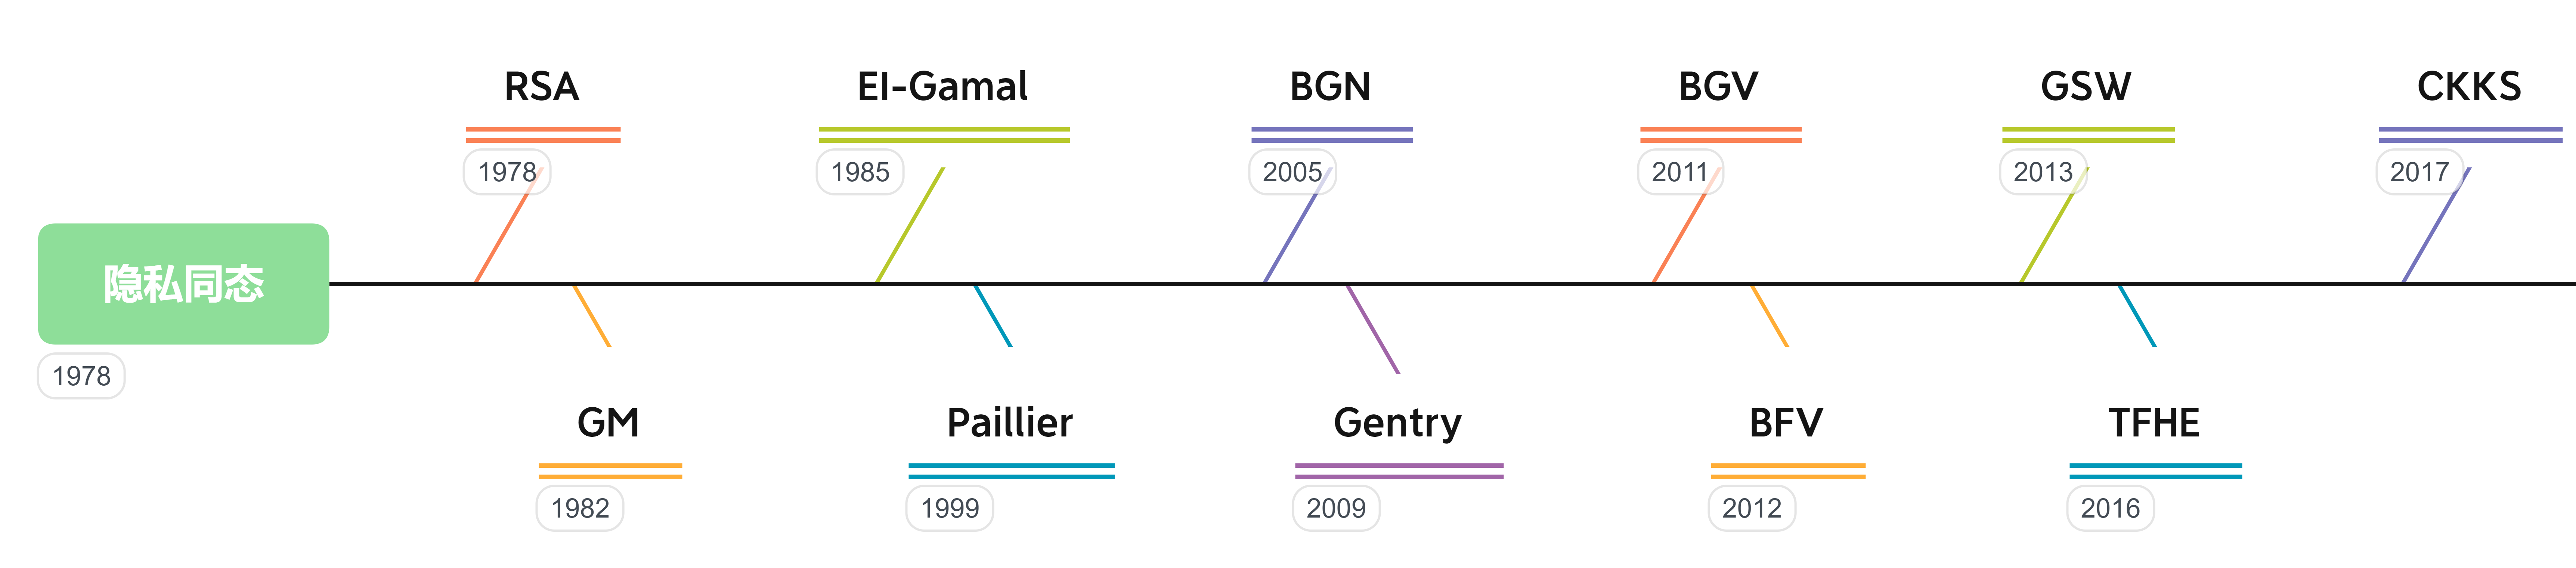
\includegraphics[scale=0.10]{img/he-timeline.png}
	\caption{同态加密发展时间线}
	\label{timeline}
\end{figure}

同态加密可以进一步细分为三类,分别是部分同态加密(Partially Homomorphic Encryption,PHE)、类同态加密(Somewhat Homomorphic Encryption,SWHE)以及全同态加密(Fully Homomorphic Encryption,FHE)。三者的区别如下表\ref{s1-table-he}所示:

\begin{table}[htbp]
	\renewcommand{\arraystretch}{1.3}
	\caption{同态加密方案对比}
	\label{s1-table-he}
	\scalebox{0.9}{
		\begin{tabular}{c|c|c|c}
			\hline
			同态加密类型 & 支持的操作类型 & 操作次数 & 常见加密方案                                   \\
			\hline
			PHE          & 加法或乘法     & 无限次   & RSA、Goldwasser-Micali、El-Gamal以及Paillier等 \\
			\hline
			SWHE         & 加法和乘法     & 有限次   & BGN                                            \\
			\hline
			FHE          & 加法和乘法     & 无限次   & GH11                                           \\
			\hline
		\end{tabular}	
	}
\end{table}


%同态加密(Homomorphic Encryption)是由Rivest、Adleman和Dertouzos于1978年首次提出的一种加密方法\cite{rivest1978data},Craig Gentry于2009年首次实现了一种可行的全同态加密方案\cite{gentry2009fully}。同态加密的发展时间线如下图\ref{timeline}所示\cite{acar2018survey}:
%
%\begin{figure}[htbp]
%	\centering
%	%	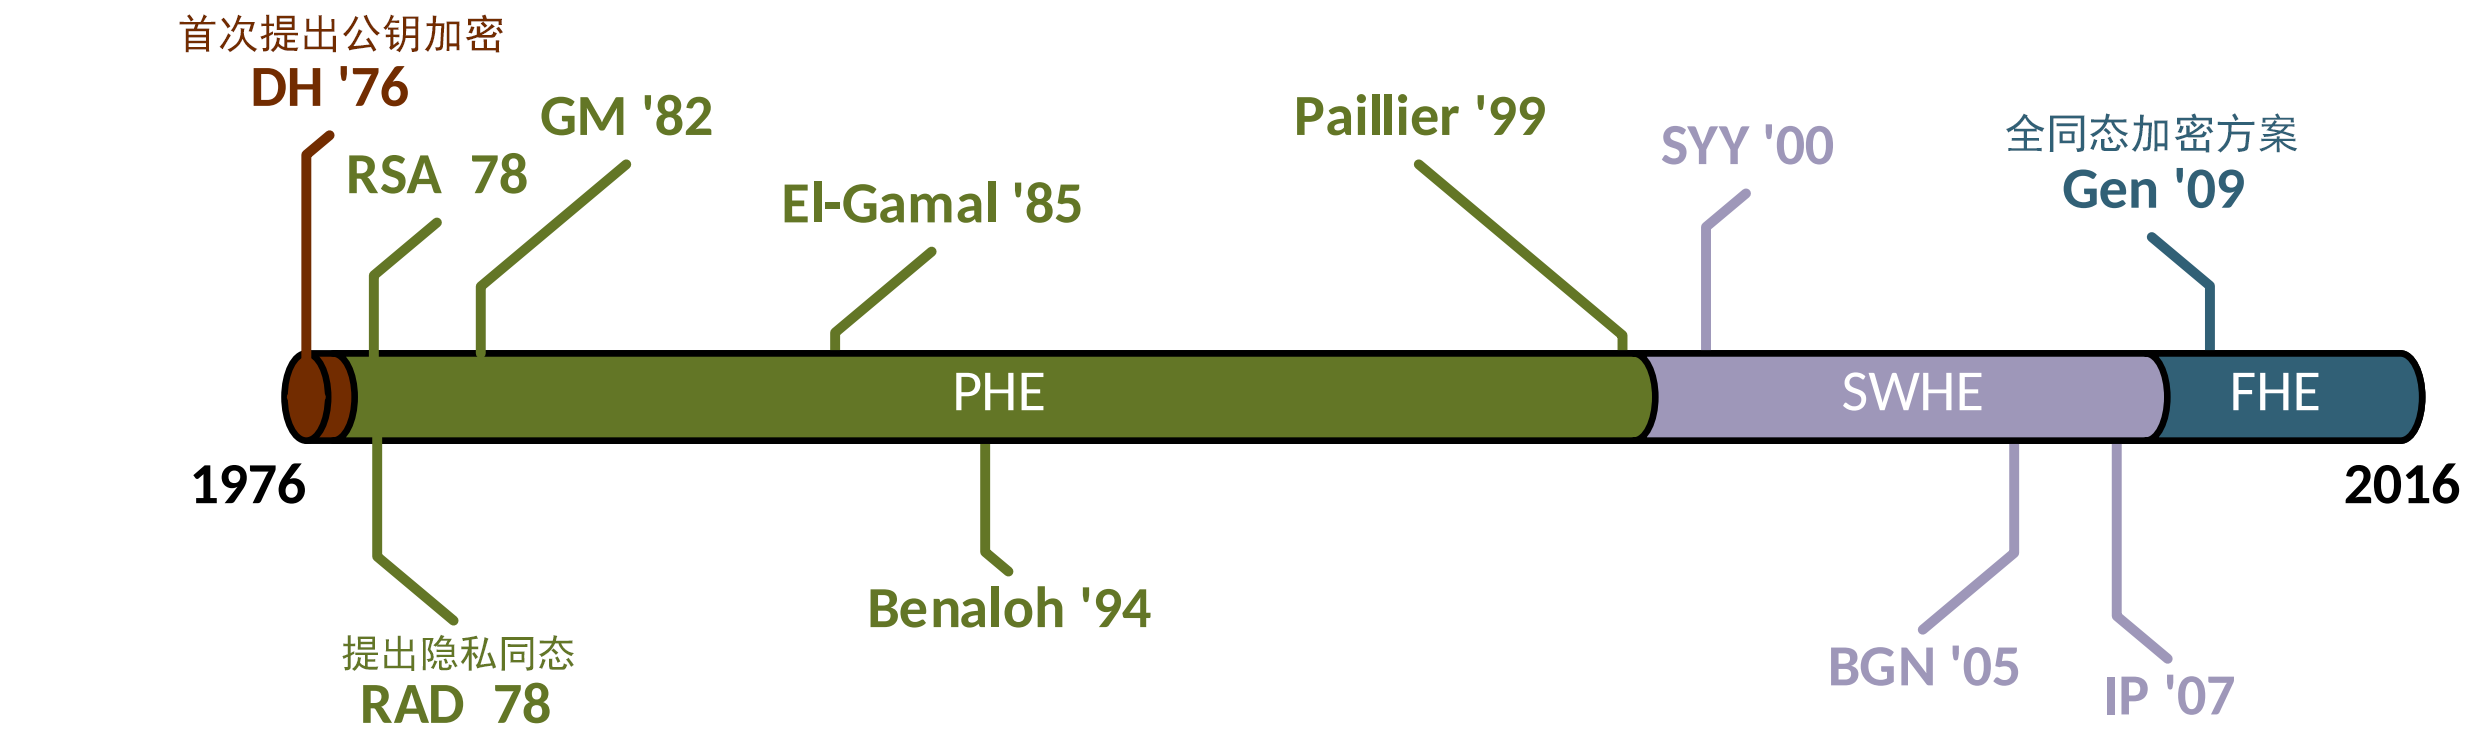
\includegraphics[scale=1.0\linewidth]{img/timeline.png}%width=\line/width
%	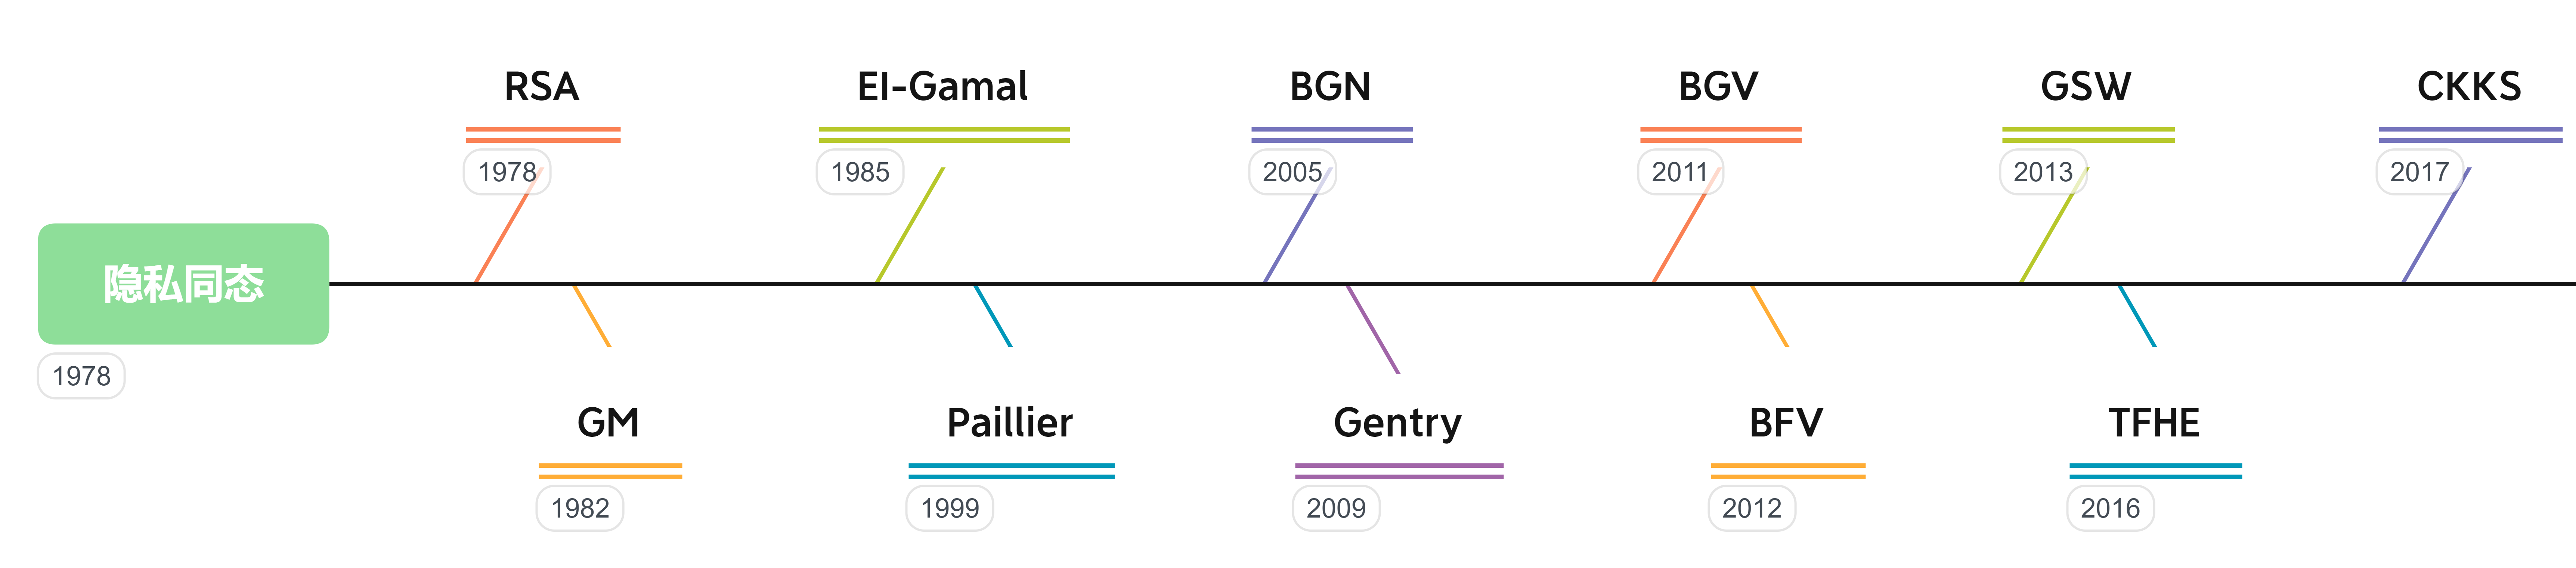
\includegraphics[scale=0.10]{img/he-timeline.png}
%	\caption{同态加密发展时间线}
%	\label{timeline}
%\end{figure}
%
%和经典的加密方式不同的是,同态加密允许直接在加密数据上进行计算,而不需要访问密钥。计算的结果仍然处于加密状态,并且可以通过密钥解密还原计算后的明文结果,目前同态加密相关研究已经取得了诸多成果。其具体定义如下:
%
%\begin{definition}
%	若一个加密方案支持如下公式,则称为操作$ \star $上的同态
%	\begin{equation}
%		D(E\left(m_1\right) \star E\left(m_2\right))=D(E\left(m_1 \star m_2\right)), \quad \forall m_1, m_2 \in M
%	\end{equation}
%
%	其中$ E() $为加密运算,$ D() $为解密运算,$ M $为所有可能信息的集合。
%\end{definition}
%
%同态加密可以进一步细分为三类,分别是部分同态加密(Partially Homomorphic Encryption,PHE)、类同态加密(Somewhat Homomorphic Encryption,SWHE)以及全同态加密(Fully Homomorphic Encryption,FHE)。三者的区别如下表\ref{s1-table-he}所示:
%
%\begin{table}[htbp]
%	\renewcommand{\arraystretch}{1.3}
%	\caption{同态加密方案对比}
%	\label{s1-table-he}
%	\scalebox{0.9}{
%	\begin{tabular}{c|c|c|c}
%	\hline
%	同态加密类型 & 支持的操作类型 & 操作次数 & 常见加密方案                                   \\
%	\hline
%	PHE          & 加法或乘法     & 无限次   & RSA、Goldwasser-Micali、El-Gamal以及Paillier等 \\
%	\hline
%	SWHE         & 加法和乘法     & 有限次   & BGN                                            \\
%	\hline
%	FHE          & 加法和乘法     & 无限次   & GH11                                           \\
%	\hline
%\end{tabular}	
%\end{table}

%\begin{compactitem}
%	\item \textbf{部分同态加密:}Partially Homomorphic Encryption(PHE)支持在密文上进行同一类型的操作无数次,该操作为加法或者乘法。常见的加密方案包括RSA、Goldwasser-Micali、El-Gamal以及Pallier等。
%	\item \textbf{类同态加密:}Somewhat Homomorphic Encryption(SWHE)支持对密文进行有限次的任意操作。常见的加密方案有BGN。
%	\item \textbf{完全同态加密:}Fully Homomorphic Encryption(FHE)支持对密文进行无限次任意操作,并且输出结果仍在密文空间内。常见的加密方案有Gentry等人\cite{gentry2011implementing}提出的GH11等。
%\end{compactitem}

同态加密目前已有诸多应用,例如加密搜索,即在同态加密的基础上使搜索引擎不知道用户搜索真正内容的前提下获取搜索结果。
安全求交,也称为隐私集合求交,该技术允许多个参与方在不公开各自数据的前提下,协同查找出交集数据,且不泄露交集数据以外的隐私信息。
多方联合建模能够在不泄露任何隐私的前提下,结合多方数据建模以提高模型效果,例如医疗机构协同诊断和银行联合反欺诈等等。

同态加密具有诸多优点,在不受信任的环境下(例如云环境或者第三方)仍能保证数据的安全性,消除了数据可用性与数据安全之间的平衡问题,无需为了数据的隐私而放弃任何数据特征,以及能够抵御量子攻击。

同态加密经过数十年的发展,从最初的半同态加密方案到现在提出的全同态加密方案,已经取得了长足进展,能够满足不同应用场景和复杂计算需求,但是由于该加密方案计算开销较大导致效率较低,仍然难以广泛应用于实际生产环境中,性能仍有很大的优化空间。

\subsubsection{安全多方计算}
安全多方计算(Secure Multi-Party Computation,SMPC)允许多个参与方之间协同进行安全的计算操作,而不泄露私有数据。每个参与方都只能看到自己输入的内容,无法获知其他参与方的输入。安全多方计算与外包计算的不同之处在于,协议的执行者同时也是数据的拥有者\cite{2018A}。

安全多方计算已经有诸多隐私保护应用,例如姚式百万富翁问题\cite{1982Protocols}、安全拍卖、投票、安全机器学习\cite{2017Oblivious}等。其中主流技术包括不经意传输(Oblivious Transfer,OT)、混淆电路(Garbled Circuits,GC)以及秘密共享(Secret Sharing,SS)。上述技术的具体介绍如下:
\begin{compactitem}
	\item \textbf{不经意传输:}是安全计算协议中一个非常重要的基础模块。标准的1-out-of-2 OT的定义涉及两方,发送方$ S $持有两个秘密$ x_0,x_1$,接收方$ R $持有一个选择比特$ b\in\{0,1\} $。不经意传输允许$ R $获得$ x_b $,同时不知道$ x_{1-b} $的内容,$ S $无法得知$ R $获得了什么内容。不经意传输技术能够应用于多种场景中,但是存在计算成本较高等问题,目前已有多种研究提出了改进方案。
	\item \textbf{混淆电路:}是最广为人知的多方计算技术。有许多协议和方案都是基于混淆电路设计,适用于各种计算操作,包括简单的加法乘法以及复杂的比较排序等。但是混淆电路计算成本相对较高,需要每个参与方进行大量通信,因此通信开销相对较大,同时设计协议比较复杂。目前许多研究工作从降低通信开销\cite{goyal2008efficient}、减少电路执行时间\cite{malkhi2004fairplay}以及减少电路门数\cite{pinkas2009secure}等角度来优化混淆电路的使用。
	\item \textbf{秘密共享:}是一种将原始信息划分为$n$个部分,分配给不同的参与方,只有满足$t$个参与方合作才能恢复出原始秘密信息的重要密码学技术。基于秘密共享的复杂安全协议,通常需要参与方之间进行频繁通信,带来较大通信开销,限制了方案的可扩展性。为了能够扩展到多个参与方的场景,一些研究工作借助大数据计算框架进行并行计算以提升效率减少通信开销。
\end{compactitem}

自安全多方计算被提出后,已经取得了长足进展,部署多方计算的开销下降了3-9个数量级。但是除了上述进展,在多方计算被大规模用于隐私保护应用之前还需要解决几个主要挑战。
\begin{compactitem}
	\item \textbf{计算和通信开销:}多方计算协议的开销跨度非常大,从几乎可忽略到实际应用难以接受,主要取决于设定的威胁模型以及实现功能的复杂程度。通常数据中心内部的带宽费用非常低,但是实际情况下,隐私保护方案的设计会将计算外包给不同的云服务提供商以防止数据被窃取,因此带宽开销不可忽视。此外,复杂协议通常需要消耗大量计算资源,耗时较长。
	\item \textbf{安全与效率权衡:}目前有一些研究选择在安全和效率之间折中。通过在核心协议中放弃一些强安全性保证来获取效率的极大提升。但是牺牲安全性保证会带来多大的数据安全问题仍有待研究。
\end{compactitem}

在表格\ref{s1-table-pet}中,总结归纳了几种不同的隐私保护技术的特点。随着研究的深入,越来越多学者提出了结合多种不同隐私保护技术的方案,扬长避短并取得了不错的成果\cite{2015ABY,jagannathan2005privacy,su2007privacy,bozdemir2021privacy}。

\begin{table}[htbp]
	\centering
	\renewcommand{\arraystretch}{1.3}
	\caption{隐私保护技术对比}
	\label{s1-table-pet}
	\scalebox{0.95}{
		\begin{tabularx}{\textwidth}{c|X|X|X|X}
			\hline  % 在表格最上方绘制横线
			技术名称     & \multicolumn{1}{c|}{特点}  & \multicolumn{1}{c|}{优点}  & \multicolumn{1}{c|}{缺点}  & \multicolumn{1}{c}{应用场景}       \\%&SKD
			\hline % 在表格最下方绘制横线
			差分隐私     & 添加噪声扰动数据           & 隐私性好,效率高           & 影响数据质量,可用性不高   & 算力较弱,对数据精度要求较低的场景 \\
			\hline
			同态加密     & 允许在密文上进行计算       & 保护数据安全               & 计算开销大,复杂计算效率低 & 算力较强,隐私保护要求高           \\
			\hline
			安全多方计算 & 数据持有方协同进行隐私计算 & 保护数据安全,计算结果准确 & 通信开销大,效率较低       & 分布式场景                         \\
			\hline
		\end{tabularx}
	}
\end{table}

\subsection{隐私保护聚类方案设计目标}
%目标是准确性、安全性、高效性
云环境下设计隐私保护聚类系统要实现的目标主要有以下三点:
\begin{compactitem}
	\item \textbf{准确性:}用户使用秘密共享、同态加密等技术处理数据后上传到云平台进行聚类,虽然保障了数据的隐私安全,但是对聚类方案的设计带来了挑战。准确性要求在密文的基础上设计系列协议实现聚类的功能,最后得到和明文一致的准确结果。
	\item \textbf{安全性:}输入数据、计算中间结果以及输出结果均与数据安全息息相关。一旦某一个环节出现问题,都可能会导致隐私被泄露,带来巨大损失。因此隐私保护聚类方案要保护数据以及所有相关结果的安全性。外包计算场景中,执行协议的云服务器应当无法窥视数据。联合数据进行训练获取结果的每个用户应无法获取其他用户的私密数据。
	\item \textbf{高效性:}随着互联网快速发展,用于聚类的数据量日益增加。在明文上进行聚类的耗时和开销已不可忽视,隐私保护方案通常计算和通信更加复杂,因此会进一步降低效率。除了要设计云平台可以高效执行的隐私保护方案,还要照顾到资源有限的用户,尽量降低用户的计算和通信开销。
\end{compactitem}

上述三个目标中,安全性与高效性通常难以同时兼顾,需要设计复杂的计算协议来实现完全安全的方案,而复杂协议则会带来不可忽视的开销。一些隐私保护工具会损失数据的准确性,但是带来效率的提升,例如差分隐私技术。在设计方案时需要综合考虑,结合应用场景和实际需求,在三者之间做出取舍,达到平衡。
\section{研究内容和创新点}
云环境下的隐私保护聚类系统,需要兼顾效率与安全。本文针对当前研究中存在的数据泄露、聚类效率低以及聚类方式单一等问题,面向具体的应用场景,基于常见聚类算法与隐私保护技术构建方案。
本文主要研究内容以及创新点如下:
\subsection{隐私保护外包K-means聚类方案研究}
K-means是机器学习算法中最为常见和流行的一种无监督聚类算法,常用于数据挖掘分析和特征提取。因其包含的计算简单,便于实现,基于K-means的隐私保护聚类方案研究较多,种类丰富。
然而现有的隐私保护K-means研究中,通常难以兼顾效率与安全,以近几年的前沿研究为例,高效的方案泄露了数据分布特点\cite{wu2020secure},完全安全的方案则效率过低\cite{jaschke2019unsupervised}。本文在论文\cite{kanungo2002efficient}的基础上,提出了一种利用Kd-tree数据结构提升效率同时保障数据安全的隐私保护外包K-means聚类方案。

在本文的方案中,用户首先在本地基于明文数据构建Kd-tree,通过秘密共享加密数据结构后分别上传至双云服务器,而后云服务器协同执行一系列安全协议,最终获得密文聚类结果。方案的创新点主要包括:(1)基于秘密共享技术和百万富翁协议\cite{rathee2020cryptflow2}构建了一系列安全计算协议,使得云平台可以在密文上完成比较、计算欧式距离以及求解极值等运算;(2)与传统K-means算法不同,本文利用Kd-tree数据结构进行计算加速,提出一种全新的隐私保护方案;(3)与现有同类工作对比,本文的计算与通信开销均较小。

\subsection{隐私保护DBSCAN相关方案研究}
K-means聚类过程简单,因此相关的隐私保护方案研究也非常丰富,但是K-means对数据集以及参数初始化有较高要求,需要人工评估簇个数$ k $,同时在非球形数据集上聚类表现较差、对异常数据比较敏感以及适用场景有限。
此外,本文提出的隐私保护外包K-means方案的应用场景为某一个用户持有所有原始数据,不支持多用户共同上传数据训练。
为了解决上述问题,本文基于另一种聚类算法,即DBSCAN,展开研究,针对不同的应用场景和实际需求提出了系列隐私保护DBSCAN方案。DBSCAN算法具有诸多优点,应用场景广泛,包含计算比较简单,对该算法进行隐私保护实现具有较大现实意义。

\subsubsection{隐私保护DBSCAN方案}
\label{fanganyi}
在传统明文DBSCAN方案\cite{1996A}的基础上,已有一些隐私保护方案的研究\cite{2006Privacy,2021Privacy},但是方案大多效率较低且开销较大,同时没有详细的实验验证和分析过程。本文结合密度聚类算法的特点对聚类过程进行重新设计,构建了一个高效的隐私保护DBSCAN方案。

协同聚类的用户各自将数据进行秘密共享后,分别发送给不共谋的双云服务器,两个云平台协同运行安全协议,并将计算结果返回给用户。用户恢复明文后,运行简单的还原算法来获取最终的聚类结果。本文提出的隐私保护DBSCAN方案的创新点主要有:(1)提出一种全新的隐私保护DBSCAN的实现方式,构建临时簇来降低迭代轮次,将部分简单的结果还原工作移交给用户以提升效率;(2)允许多个独立的参与方上传数据进行协同聚类,在不知道彼此数据的前提下获取最终聚类结果;(3)极大程度上提升了效率,耗时减少近100倍。
\subsubsection{改进的隐私保护DBSCAN方案}
明文DBSCAN方案存在聚类结果不稳定的问题,若数据同时满足被划分到多个簇的条件,则最终的划分结果取决于数据遍历的顺序,打乱顺序后再次排序可能得到不同的结果。论文\cite{tran2013revised}提出了一种修改后的明文DBSCAN方案以获取稳定的聚类结果。本文在上述论文的基础上设计了一种改进的隐私保护DBSCAN方案,能够获取稳定的密文划分结果,提升密文聚类质量。
%因此本文在论文\cite{tran2013revised}的基础上,提出了一种改进的隐私保护DBSCAN方案。

方案的实现流程可以分为初始化,聚类以及还原结果三步。主要的创新点有:(1)针对结果稳定性问题首次提出隐私保护方案;(2)在优化聚类效果的基础上,效率远高于目前的同类方案\cite{bozdemir2021privacy},耗时缩短近20倍。

\subsubsection{基于DBSCAN的隐私保护层次聚类方案}
DBSCAN聚类的效果受到关键参数的影响,而参数的设置需要分析数据分布特点,在多用户各自持有数据的场景下难以找到合适的方法确定参数值。同时,对于包含不同密度的数据集,传统DBSCAN方案难以获取合理的聚类结果,可能出现较小簇或者单个点的情况。为了解决上述问题,论文\cite{latifi2021dbhc}在明文上,利用k线图和k近邻算法获取关键参数,进行多轮聚类以获取划分结果。本文在上述论文的基础上提出了一种基于DBSCAN的隐私保护层次聚类方案,能够在密文上获取聚类关键参数,并获取最终划分结果。
%本文基于论文\cite{latifi2021dbhc}的思想,借助$ k $线图和$ k $近邻算法,提出了一个基于DBSCAN的隐私保护层次聚类方案。

方案分为获取eps值、计算初始簇以及合并初始簇还原结果三个步骤。用户上传加密数据到双云服务器后,云平台通过执行系列给定的安全协议,获取最终结果并发送给用户。本方案的创新点主要有:(1)基于秘密共享设计了安全排序协议;(2)无需人工给出关键参数,减少用户计算开销;(3)适应包含不同密度数据的数据集,应用更加广泛。

\section{论文组织结构}

本文主要分为5个章节,组织结构如图\ref{lunwenjiegou}所示。
\begin{figure}[htbp]
	\centering
	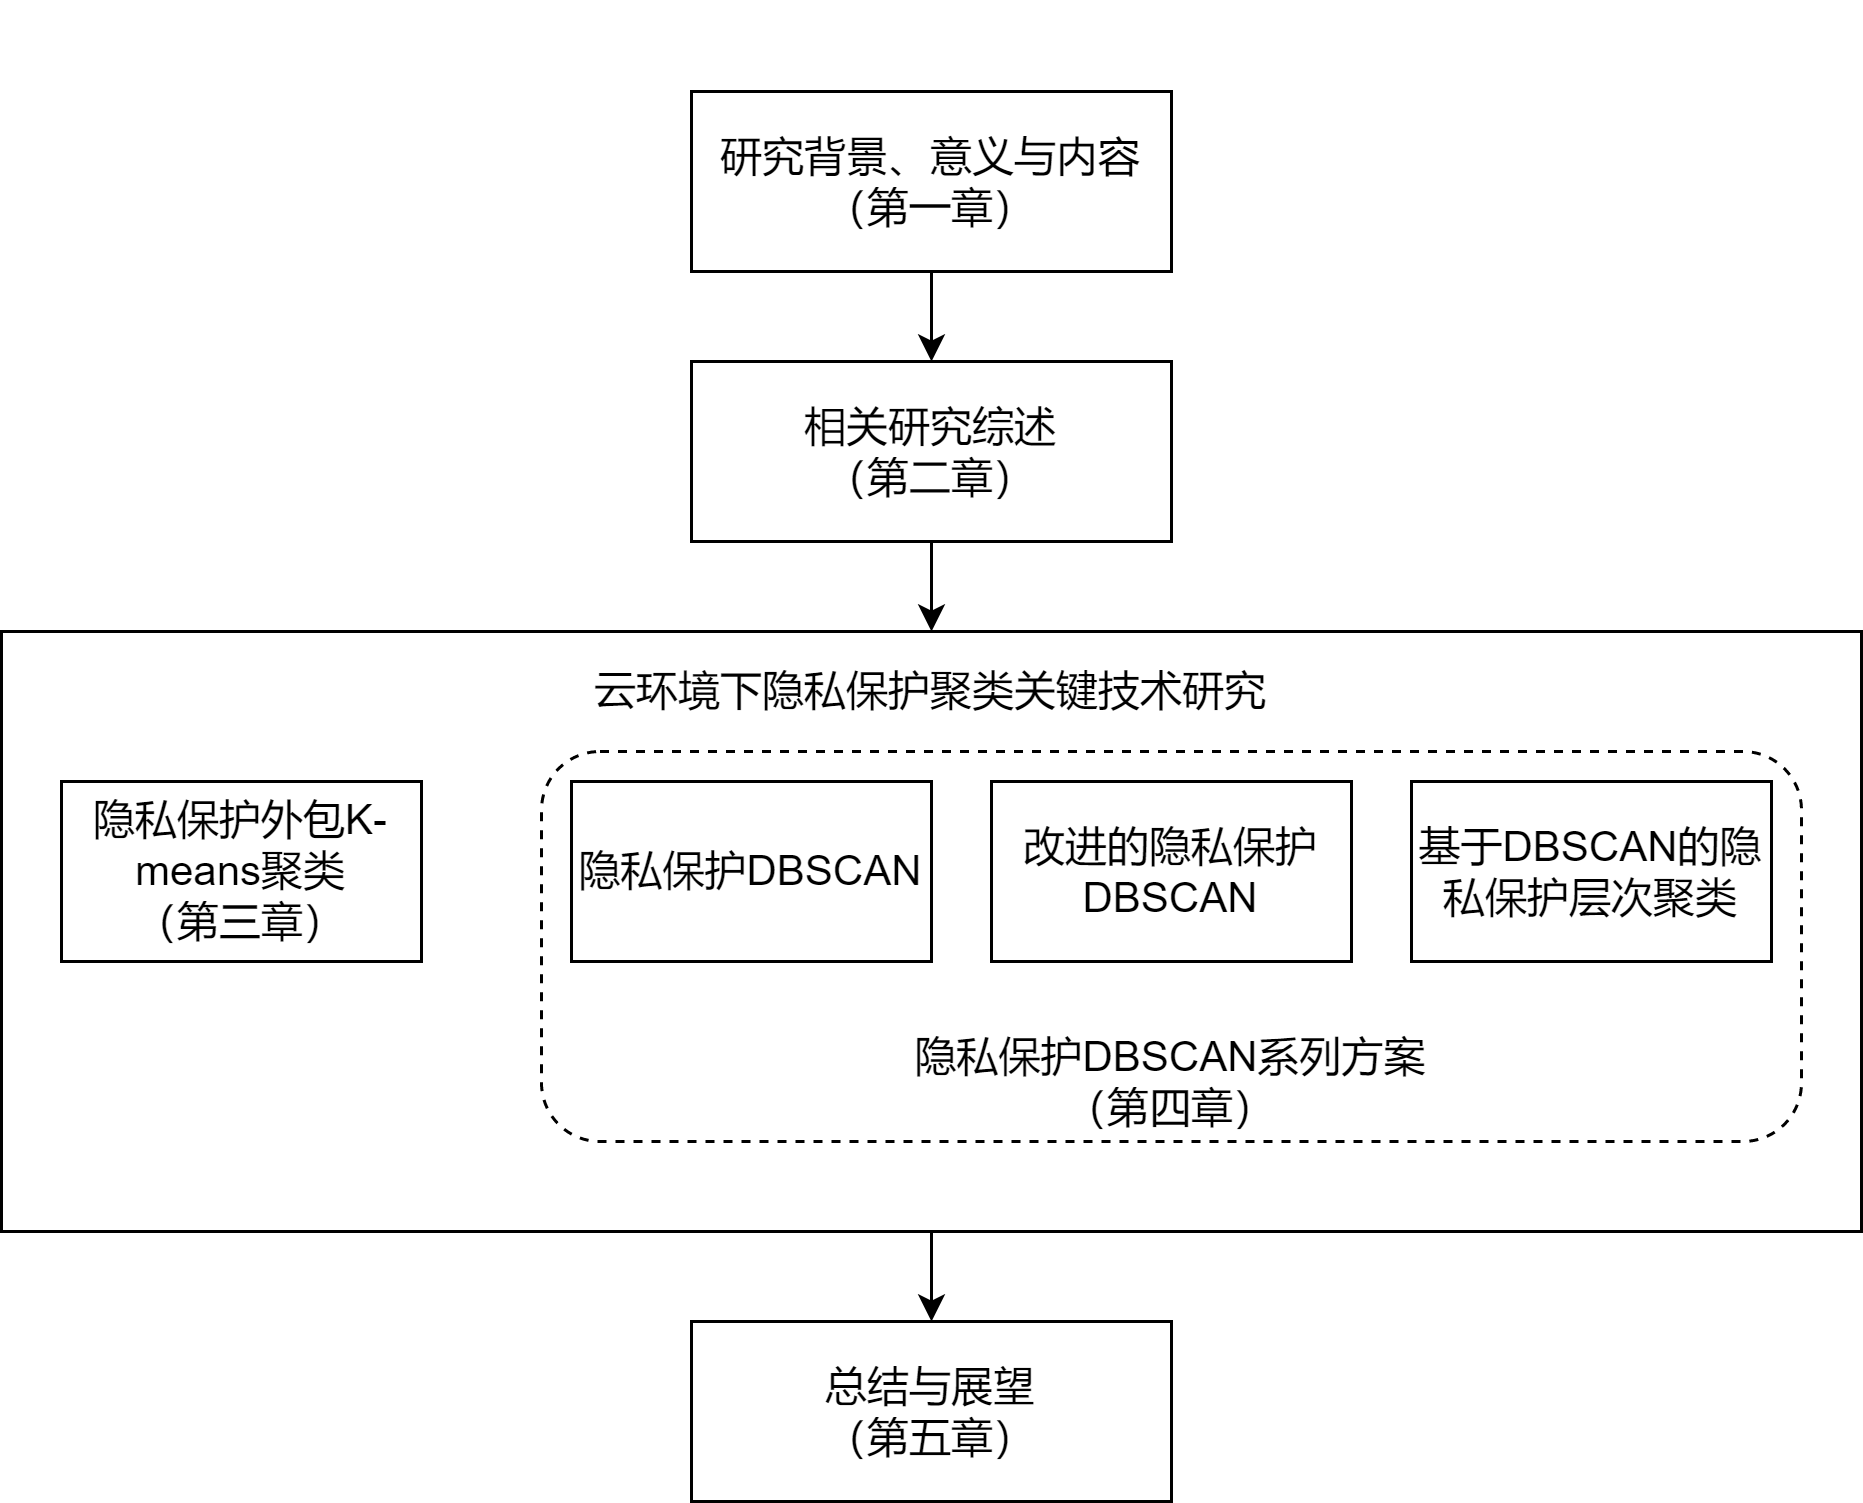
\includegraphics[scale=0.9]{img/dd.png}%width=\linewidth
	\caption{论文组织结构}
	\label{lunwenjiegou}
\end{figure}

第一章是绪论,首先介绍了云计算和聚类的基本概念,通过剖析云环境下聚类的发展应用,引出了研究云环境下聚类所面临的数据安全和效率问题的意义,然后概述了设计隐私保护聚类方案可能利用的密码学技术及其优缺点,并给出了隐私保护聚类系统的设计目标。最后,简要介绍了本文的主要工作与贡献。

第二章是相关研究综述。本章调研了近年来隐私保护K-means方案以及隐私保护DBSCAN方案的相关研究,通过横向以及纵向对比,总结归纳了不同方案的优缺点。

第三章是隐私保护外包K-means聚类方案。现有的隐私保护K-means聚类方案大多无法兼顾效率与数据安全。为了在保证安全的基础上提升效率,减少用户的计算和通信开销,本文借助Kd-tree数据结构,基于秘密共享设计了一系列安全协议,实现了安全高效的聚类方案。通过安全性分析、理论分析以及全面的实验评估,验证了方案的有效性和安全性,以及高效率。

第四章是隐私保护密度聚类方法研究。针对K-means聚类中存在的各种问题,提出了系列基于DBSCAN的隐私保护聚类方案,分别解决了K-means不适合非凸样本簇、传统DBSCAN聚类结果不稳定以及传统DBSCAN不适合多密度数据集的问题。通过系列分析,验证了方案的正确性、安全性和高效性。

第五章是总结与展望。本章首先总结了本文的研究工作,然后基于此对未来工作进行了展望。

